\newcommand{\convexA}{
  \coordinate (p0) at (4.5,2);
  \coordinate (p1) at (4,3.25);
  \coordinate (p2) at (2,4);
  \coordinate (p3) at (1,3.5);
  \coordinate (p4) at (0,2);
  \coordinate (p5) at (2,0);
  \coordinate (p6) at (3.75,1);

  \draw (p0) -- (p1) -- (p2) -- (p3) -- (p4) -- (p5) -- (p6) -- cycle;
}

\newcommand{\convexB}{
  \coordinate (p0) at (3.5,     4);
  \coordinate (p1) at (1.5,     4.5);
  \coordinate (p2) at (0,       3.5);
  \coordinate (p3) at (-0.5,    1.5);
  \coordinate (p4) at (1.75,    0);
  \coordinate (p5) at (4,       1);

  \draw (p0) -- (p1) -- (p2) -- (p3) -- (p4) -- (p5) -- cycle;
}

\newcommand{\nonconvex}{
  \coordinate (p0) at (4.5,2);
  \coordinate (p1) at (2,4);
  \coordinate (p2) at (0,3);
  \coordinate (p3) at (1.5,2);
  \coordinate (p4) at (2,0);
  \coordinate (p5) at (3,1.5);

  \draw (p0) -- (p1) -- (p2) -- (p3) -- (p4) -- (p5) -- cycle;
}

\chapter{Lokalizacja punktu\label{chap:point_location}}
Problem lokalizacji punktu sformułowany jest następująco.

\begin{problem}[Lokalizacja punktu]
  Jeśli dany jest wielokąt prosty $P$ i punkt $z$ na płaszczyźnie
  $\mathbb{R}^2$, sprawdzić, czy punkt $z$ należy do $P$.
\end{problem}

Problem ten można rozwiązać w czasie liniowym bez przetwarzania
wstępnego. Rozważmy poziomą prostą $l$ przechodząca przez punkt
$z$. Musimy rozważyć kilka przypadków.

Jeśli $l$ nie przecina $P$, to $z$ leży na zewnątrz wielokąta
(rysunek~\ref{fig:location1}).

\begin{figure}[htp]
  \centering
  \begin{tikzpicture}
    \nonconvex

    \node [anchor=center,circle,draw,fill,inner sep=0.5pt,
    label={right:$p_0$}] at (p0) {};

    \node [anchor=center,circle,draw,fill,inner sep=0.5pt,
    label={above:$p_1$}] at (p1) {};

    \node [anchor=center,circle,draw,fill,inner
    sep=0.5pt,label={left:$p_2$}] at (p2) {};

    \node [anchor=center,circle,draw,fill,inner
    sep=0.5pt,label={190:$p_3$}] at (p3) {};

    \node [anchor=center,circle,draw,fill,inner
    sep=0.5pt,label={below:$p_4$}] at (p4) {};

    \node [anchor=center,circle,draw,fill,inner
    sep=0.5pt,label={300:$p_5$}] at (p5) {};

    \coordinate (z) at (2.5,-1);
    \coordinate (l) at (-1,-1);

    \draw [shorten >=-3cm, shorten <=-1cm] (l) -- (z);

    \node [anchor=center,circle,draw,fill,inner
    sep=0.5pt,label={below:$z$}] at (z) {};

    \node [label={[label distance=0.3cm]177:$l$}] at (l) {};
  \end{tikzpicture}
  \caption{\label{fig:location1}}
\end{figure}

W przypadku, gdy prosta $l$ przecina $P$ i nie przechodzi przez
żaden z wierzchołków $P$, oznaczmy przez $p_l$ liczbę przecięć $l$ z
wielokątem $P$. Wiemy, że lewy koniec $l$ leży na zewnątrz $P$, więc
przesuwając się po prostej $l$ w prawo w kierunku $z$ i przecinając
brzeg wielokąta, przechodzimy do jego wnętrza. Przy następnym
przecięciu z brzegiem $P$ znowu znajdziemy się na zewnątrz
itd. Widzimy stąd, że $z$ jest na zewnątrz wielokąta $P$ wtedy i
tylko wtedy, gdy $p_l$ jest parzyste (rysunek~\ref{fig:location2}).

\begin{figure}[htp]
  \centering
  \begin{tikzpicture}
    \nonconvex

    \node [anchor=center,circle,draw,fill,inner sep=0.5pt,
    label={right:$p_0$}] at (p0) {};

    \node [anchor=center,circle,draw,fill,inner sep=0.5pt,
    label={above:$p_1$}] at (p1) {};

    \node [anchor=center,circle,draw,fill,inner
    sep=0.5pt,label={left:$p_2$}] at (p2) {};

    \node [anchor=center,circle,draw,fill,inner
    sep=0.5pt,label={190:$p_3$}] at (p3) {};

    \node [anchor=center,circle,draw,fill,inner
    sep=0.5pt,label={below:$p_4$}] at (p4) {};

    \node [anchor=center,circle,draw,fill,inner
    sep=0.5pt,label={300:$p_5$}] at (p5) {};

    \coordinate (z) at (2.5,2.5);
    \coordinate (l) at (-1,2.5);

    \draw [shorten >=-3cm, shorten <=-1cm] (l) -- (z);

    \node [anchor=center,circle,draw,fill,inner
    sep=0.5pt,label={below:$z$}] at (z) {};
    \node [label={[label distance=0.3cm]177:$l$}] at (l) {};
  \end{tikzpicture}
  \caption{\label{fig:location2}}
\end{figure}

Szczególnym przypadkiem jest ten, w którym $l$ przechodzi przez jeden
lub dwa wierzchołki. W algorytmie rozważamy przecięcia $l$ z
krawędziami $P$, więc musimy się zabezpieczyć przed sytuacją, w której
policzylibyśmy przecięcie brzegu $P$ dwukrotnie. Stosujemy tu zasadę,
że $p_l$ zostanie zwiększone dla przecinanej krawędzi, której jeden z
wierzchołków znajduje się powyżej prostej $l$. Zauważmy, że w
przypadku, gdy prosta $l$ przechodzi przez oba wierzchołki krawędzi
$e$ wielokąta, przecięcie z $e$ nie jest zliczane.

\begin{figure}[htp]
  \centering
  \begin{tikzpicture}
    \nonconvex

    \node [anchor=center,circle,draw,fill,inner sep=0.5pt,
    label={below:$p_0$}] at (p0) {};

    \node [anchor=center,circle,draw,fill,inner sep=0.5pt,
    label={above:$p_1$}] at (p1) {};

    \node [anchor=center,circle,draw,fill,inner
    sep=0.5pt,label={left:$p_2$}] at (p2) {};

    \node [anchor=center,circle,draw,fill,inner
    sep=0.5pt,label={190:$p_3$}] at (p3) {};

    \node [anchor=center,circle,draw,fill,inner
    sep=0.5pt,label={below:$p_4$}] at (p4) {};

    \node [anchor=center,circle,draw,fill,inner
    sep=0.5pt,label={300:$p_5$}] at (p5) {};

    \coordinate (z) at (2.5,2);
    \coordinate (l) at (-1,2);

    \draw [shorten >=-3cm, shorten <=-1cm] (l) -- (z);

    \node [anchor=center,circle,draw,fill,inner
    sep=0.5pt,label={below:$z$}] at (z) {};
    \node [label={[label distance=0.3cm]177:$l$}] at (l) {};
  \end{tikzpicture}
  \caption{Przecięcie zostanie policzone dla krawędzi $p_{2}p_{3}$
    oraz $p_{0}p_{1}$.}
\end{figure}

Ze względu na to, że każdą krawędź $P$ sprawdzamy tylko raz
pod względem przecięcia z $l$, mamy do czynienia ze złożonością
liniową zależną od liczby krawędzi wielokąta.

Algorytm dla wielokąta wypukłego wymaga przetwarzania wstępnego, ale
jest użyteczny w przypadku wykonywania wielokrotnych zapytań o
przynależność punktu do danego wielokąta. Weźmy punkt $q$ leżący
wewnątrz wielokąta wypukłego $P$ o $N$ wierzchołkach, może to być na
przykład środek ciężkości trójkąta wyznaczony przez trzy dowolne jego
wierzchołki, a następnie poprowadźmy $N$ półprostych z $q$
przechodzących przez wierzchołki $P$. Płaszczyzna wraz z wielokątem
zostaje podzielona na $N$ części, które nazywamy \emph{klinami}, z
których każdy jest podzielony przez krawędź $P$ na dwie części ---
jest to wnętrze i zewnętrze wielokąta (rysunek~\ref{fig:location3}).

\begin{figure}[htp]
  \centering
  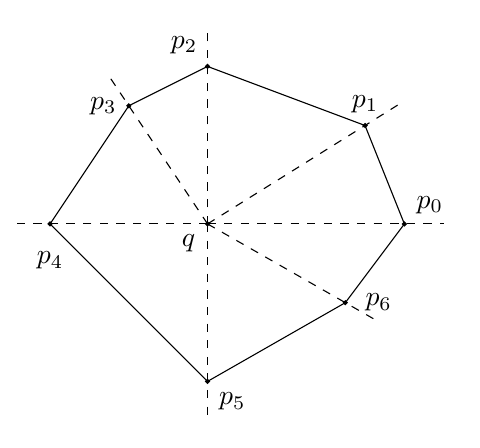
\begin{tikzpicture}
    \convexA

    \node [anchor=center,circle,draw,fill,inner sep=0.5pt,
    label={10:$p_0$}] at (p0) {};

    \node [anchor=center,circle,draw,fill,inner sep=0.5pt,
    label={90:$p_1$}] at (p1) {};

    \node [anchor=center,circle,draw,fill,inner
    sep=0.5pt,label={100:$p_2$}] at (p2) {};

    \node [anchor=center,circle,draw,fill,inner
    sep=0.5pt,label={180:$p_3$}] at (p3) {};

    \node [anchor=center,circle,draw,fill,inner
    sep=0.5pt,label={[label distance=0.2cm]-90:$p_4$}] at (p4) {};

    \node [anchor=center,circle,draw,fill,inner
    sep=0.5pt,label={-45:$p_5$}] at (p5) {};

    \node [anchor=center,circle,draw,fill,inner
    sep=0.5pt,label={[label distance=0.1cm]0:$p_6$}] at (p6) {};

    \coordinate (z) at (2,2);

    \draw [dashed,shorten >=-0.5cm] (z) -- (p0);
    \draw [dashed,shorten >=-0.5cm] (z) -- (p1);
    \draw [dashed,shorten >=-0.5cm] (z) -- (p2);
    \draw [dashed,shorten >=-0.5cm] (z) -- (p3);
    \draw [dashed,shorten >=-0.5cm] (z) -- (p4);
    \draw [dashed,shorten >=-0.5cm] (z) -- (p5);
    \draw [dashed,shorten >=-0.5cm] (z) -- (p6);

    \node [anchor=center,circle,draw,fill,inner
    sep=0.5pt,label={-170:$q$}] at (z) {};
  \end{tikzpicture}
  \caption{\label{fig:location3}}
\end{figure}

W tej pracy będziemy zakładać, że brzeg wielokąta $P$ tworzą
wierzchołki $p_0, \ldots, p_{N-1}$, ponumerowane w kolejności
przeciwnej do ruchu wskazówek zegara. Wyszukiwanie położenia danego
punktu $z$ składa się z dwóch etapów. Najpierw określany jest klin, w
którym leży $z$. Można to zrobić w czasie $O(\log N)$ używając
wyszukiwania binarnego.
% % nie działa w pewnych przypadkach
% Punkt $z$ będzie znajdował się pomiędzy promieniami $p_i$ i $p_{i+n}$
% podzielonej płaszczyzny wtedy i tylko wtedy, gdy kąt $\angle p_{i}qz$
% będzie lewoskrętny, a kąt $\angle p_{i+n}qz$ prawoskrętny. W
% następnych krokach stopniowo zawężamy nasz obszar poszukiwań, do czasu
% aż odnajdziemy właściwy klin.
Następnie określamy, czy $z$ należy do wnętrza lub zewnętrza
znalezionego klinu. Jeśli kąt $\angle p_{i}p_{i+1}z$ jest lewoskrętny,
to $z$ jest wewnętrzny. Określenie skrętności kąta jest operacją o
czasie $O(1)$, więc asymptotyczna złożoność tej części algorytmu jest
rzędu $O(\log N)$.

% Umieszczenie wielokąta w strukturze danych umożliwiającej
% przeszukiwanie binarne wymaga rozważenia przypadku zobrazowanego na
% rysunku \ref{fig:binstruct}. By punkt $z$ został zakwalifikowany jako
% należący do klina $(p_{3},p_{0})$ musi leżeć na przecięciu
% półpłaszczyzny $H_1$ określonej przez obszar na prawo od prostej
% zdefiniowanej przez odcinek $p_{3}q$ oraz półpłaszczyzny $H_2$
% określonej przez obszar na lewo od prostej zdefiniowanej przez odcinek
% $p_{0}q$. W sytuacji gdy kąt klina jest kątem rozwartym punkt $z$ nie
% zostanie wykryty. Z tego powodu przy wyszukiwaniu binarnym powinniśmy
% zaczynać od klina, którego kąt wewnętrzny jest
% mniejszy. Uwzględniająca ten warunek (wiersze 4--9) procedura została
% przedstawiona na listingu \ref{alg:findwedge}.

% \begin{figure}[htp]
%   \centering
%   \begin{tikzpicture}
%     \convexB

%     \node [anchor=center,circle,draw,fill,inner sep=0.5pt,
%     label={90:$p_0$}] at (p0) {};

%     \node [anchor=center,circle,draw,fill,inner
%     sep=0.5pt,label={100:$p_1$}] at (p1) {};

%     \node [anchor=center,circle,draw,fill,inner
%     sep=0.5pt,label={180:$p_2$}] at (p2) {};

%     \node [anchor=center,circle,draw,fill,inner
%     sep=0.5pt,label={[label distance=0.2cm]-90:$p_3$}] at (p3) {};

%     \node [anchor=center,circle,draw,fill,inner
%     sep=0.5pt,label={-45:$p_4$}] at (p4) {};

%     \node [anchor=center,circle,draw,fill,inner
%     sep=0.5pt,label={[label distance=0.1cm]0:$p_5$}] at (p5) {};

%     \coordinate (q) at (2,2);
%     \coordinate (z) at (3.25,3);

%     \draw [dashed,shorten >=-0.5cm] (q) -- (p0);
%     \draw [dashed,shorten >=-0.5cm] (q) -- (p1);
%     \draw [dashed,shorten >=-0.5cm] (q) -- (p2);
%     \draw [dashed,shorten >=-0.5cm] (q) -- (p3);
%     \draw [dashed,shorten >=-0.5cm] (q) -- (p4);
%     \draw [dashed,shorten >=-0.5cm] (q) -- (p5);

%     \draw [name path=p4--q,green,dashed,shorten >=-4cm,shorten <=-2cm,->] (p3) -- (q);
%     \draw [name path=p1--q,blue,dashed,shorten >=-4cm,shorten <=-1.5cm,->] (p0) -- (q);

%     %     \path [name intersections={of=p4--q and p1--q,by=i1}];

%     %     \fill [red] ($(q)!(-2,0)!(p1)$) circle [radius=2pt];
%     %     \fill [blue] ($(q)!(11,0)!(p1)$) circle [radius=2pt];

%     \filldraw [color=blue,opacity=0.2] (6,5) --
%     ($(q)!(11,0)!(p0)$) -- ($(q)!(-2,0)!(p0)$) -- (6,-1.2);

%     %     \fill [red] ($(p4)!(-2.5,0)!(q)$) circle [radius=2pt];
%     %     \fill [red] ($(p4)!(6.5,0)!(q)$) circle [radius=2pt];

%     \filldraw [color=green,opacity=0.2] ($(p3)!(-2.5,0)!(q)$) --
%     ($(p3)!(6.5,0)!(q)$) -- (6,-1.2) -- (-2.7,-1.2);

%     \node [anchor=center,circle,draw,fill,inner
%     sep=0.5pt,label={-170:$q$}] at (q) {};
%     \node [anchor=center,circle,draw,fill,inner
%     sep=0.5pt,label={below:$z$}] at (z) {};
%   \end{tikzpicture}
%   \caption{\label{fig:binstruct}}
% \end{figure}

Zastosowane tutaj przeszukiwanie binarne jest możliwe dzięki temu, że
wierzchołki wielokąta wypukłego występują w kolejności kątowej lub
inaczej mówiąc w kolejności krążenia wokół punktu $q$. Przetwarzanie
wstępne dla wielokąta $P$, na które składa się wyznaczenie punktu $q$
oraz umieszczenie wielokąta w strukturze danych wspierającej
wyszukiwanie binarne, może zostać wykonane w czasie $O(n)$. Algorytm
wyszukiwania klina został przedstawiony za pomocą pseudokodu z
listingu~\ref{alg:findwedge}. Należy zauważyć, że indeksy wierzchołków
są wyliczane za pomocą działania \emph{modulo} $N$. Innymi słowy,
następnikiem wierzchołka $p_{N-1}$ jest wierzchołek $p_0$.

% Przyjęto także założenie, że brzeg $P$ należy do jego wnętrza.

\begin{figure}[htp]
  \begin{algorithmic}[1]
    \Procedure{Find Wedge}{}

    \State {$j \gets \lfloor N/2 \rfloor$}
    \State {$i \gets 0$}

    \State

    \If {$z$ leży w klinie $p_jqp_i$}
        \State {kontynuuj}
    \Else
        \State {$i \gets j$}
        \State {$j \gets N$}
    \EndIf

    \State

    \While {nie wyznaczono pojedynczego klina}
        \State $s \gets \lfloor (j-i)/2 \rfloor$

        \State

        \If {$z$ leży w klinie rozpiętym przez $p_sqp_i$}
                \State {$j \gets s$}
        \Else
                \State {$i \gets s$}
        \EndIf
    \EndWhile

    \State

    \State $print(p_i, p_j)$

    \EndProcedure

    \end{algorithmic}
    \caption{\label{alg:findwedge}}
  \end{figure}

  %%% Local Variables:
  %%% mode: latex
  %%% TeX-master: "masterthesis"
  %%% TeX-engine: xetex
  %%% End:
